\section{Überblick über den Optimierungsvorgang}
Die Ausführung des Programms geschieht in drei Schritten: (1) Konfiguration, (2) Generierung von semantisch gleichen Plänen, (3) Finden des optimalen Plans.

Im ersten Schritt, wird auf Grund von externen Parametern das System konfiguriert. Die Konfiguration erfolgt durch ein JSON File. In ihm werden die Parameter für die Optimierung festgelegt:

\begin{itemize}
\item Relationen und deren Kardinalität 
\item JoinEdges und deren Selektvität
\item Inital-Plan
\item Regelsets
\end{itemize}

Mit Hilfe der Relationen und deren Kardinalität kann später im Zusammenspiel mit JoinEdges und Selektvitität die Kosten für einen Plan berechnet werden. Der initale Plan dient als Startpunkt der Transformation. Auf ihn werden die Regelsets angewendet und so logisch äquivalente erzeugt.

Zu Beginn des zweiten Schritts, der Erzeugung von äquivalenten Plänen, wird die Zeitmessung gestartet.  Mit Hilfe von Exektuoren werden die unterschiedlichen Regelsets auf den Initialen Plan angewendet. Für jeden Knoten wird zuerst festgestellt, ob er bereits expanded wurde. Falls das nicht der Fall ist, wird geprüft, ob eine Regel aus dem Regelset anwendbar ist, ist das der Fall, kommt die Regel zum Einsatz. Nur wenn der neu-erzeugte Plan bisher noch unbekannt ist, wird er einer Äquivalenzklasse hinzugefügt.

In einem finalen Schritt wird findet die Kostenberechnung statt und aus den möglichen Plänen wird der günstigste ausgewählt. Diese Preisberechnung findet im Modul der Kostenschätzung statt.


\begin{figure}[h]
  \centering
  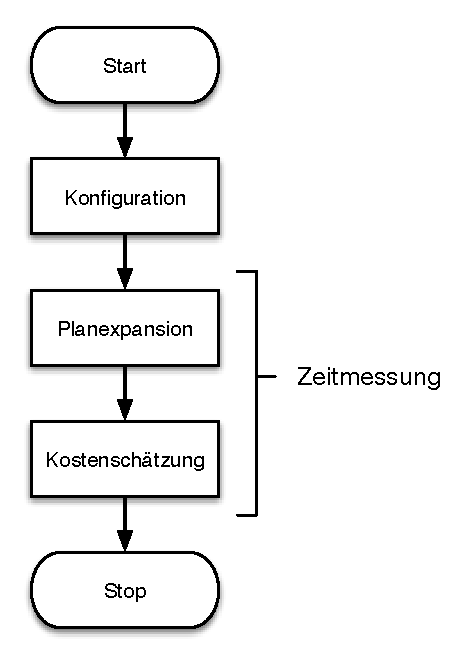
\includegraphics{04_Implementierung/Ablauf.pdf}
  \caption{Ablauf der eigenen Implementierung}
  \label{Ablauf}
\end{figure}


\subsection{Unterschiede im Ablauf zu Volcano und Pyro}